\documentclass[12pt]{article}

% Rewrite \maketitle command
\makeatletter
\def\thickhrulefill{\leavevmode \leaders \hrule height 1pt\hfill \kern \z@}
\def\maketitle{
    \null \thispagestyle{empty} 
    \vskip 1cm
    \begin{flushright}\normalfont\Large\@author\\\end{flushright}
    \vfil
    \hrule height 2pt
    \par
    \begin{center}\huge \strut \@title \par  
    \begin{scriptsize}(\@date)\end{scriptsize} 
    \end{center}
    \hrule height 2pt
    \begin{center}
\includegraphics[width=0.20\textwidth]{images/hs.png}\end{center}
    \begin{center}\huge Hochschule Ravensburg-Weingarten \\ University of Applied Sciences\end{center}
    \par \vfil \vfil \null
}
\makeatother

% Packages
\usepackage[utf8]{inputenc}  % Encoding
\usepackage[T1]{fontenc}     % Font encoding
\usepackage{graphicx}        % Include graphics
\usepackage{geometry}        % Page layout
\geometry{a4paper, margin=1in} % Set paper size and margins
\usepackage{amsmath}         % Mathematics
\usepackage{lipsum}          % Dummy text
\usepackage{setspace}        % Line spacing control
\setstretch{1.5}             % Equivalent to \linespread{1.5}
\usepackage{hyperref}        % Hyperlinks
\usepackage{listings}        % Listings
\usepackage{caption}         % Captions
\usepackage[justification=centering]{caption}  % This will center all captions


% Add biblatex package with biber as backend
\usepackage[backend=biber, style=numeric, citestyle=numeric]{biblatex}
\addbibresource{literature.bib} % Link to your bibliography file

% Provides command patching capabilities
\usepackage{etoolbox}  
\pretocmd{\section}{\cleardoublepage}{}{}

% Customized header
\usepackage{fancyhdr}
\pagestyle{fancy}
\fancyhf{} % clear all header and footer fields
\renewcommand{\headrulewidth}{0.4pt} % horizontal line under the header

\setlength{\headheight}{15pt} % Change headheight to avoid fancyhdr warnigns

\rhead{\leftmark} % Left header: only title
\renewcommand{\sectionmark}[1]{\markboth{\uppercase{#1}}{}}  % Updates leftmark with only uppercase section title
\cfoot{\thepage} % Center footer: page number

\usepackage{chngcntr}
\counterwithout{table}{section}  % Removes dependency on the section
\counterwithout{table}{subsection}  % Removes dependency on the subsection
  % Include all packages and settings

\begin{document}

% Title page
\title{Seminar Nachhaltigkeit Protokoll: KI für klimaresiliente Städte (Smart Cities)}
\author{Owusu Joseph Kwabena (15542936)\\[1ex]
Volodymyr Kryvytskyi (12042811)\\[1ex]
Supervisor: Prof. Dr. rer. nat. Markus Pfeil}
\date{\today} % or any specific date

\maketitle

% Table of contents
\tableofcontents
\setcounter{page}{1} % Resets page numbering

\section{Abstract}
There is always the constant need to improve civilization and technology, yet this advancement 
often has direct and negative effects on our environment. As we would say in economics, 
we have to make trade-offs. The challenge, therefore, is to find a crucial balance: advancing 
technology and civilization while simultaneously finding sustainable ways to protect our environment, 
especially as urban areas become increasingly vulnerable to climate-related stresses.

This seminar paper explores the frameworks of Artificial Intelligence (AI) for data-oriented 
decision-making for climate-resilient cities (Smart Cities). The analysis focuses on two core 
applications: First, the prediction of extreme weather events (Hitzewellen, Starkregen) using 
advanced AI-driven models based on satellite and real-time sensor data, aimed at establishing 
more accurate and faster early warning systems for public safety. Second, the AI-controlled 
optimization of urban infrastructure, with a specific focus on rainwater management 
to prevent flooding and intelligently manage valuable water resources.

This paper doesn't only details the technical possibilities and advantages of AI in this 
context, but through text-driven analysis of current research, international case studies, 
and expert interviews, how robust and adaptive AI systems can significantly enhance urban 
resilience to climate change. The objective is to evaluate the transformative potential of AI 
in enhancing urban resilience, explaining the evolution of these models, and outlining the necessary 
framework conditions for ecologically, economically, and socially sustainable implementation.
\section{Introduction}
\subsection{Background and Motivation}

The acceleration of climate change is a pressing challenge for global civilization: how to sustain 
technological and economic development while ensuring planetary health. This tension is nowhere more serious 
than in urban environments, which are both foundational elements of human progress and highly vulnerable center 
points for climate risks. Extreme weather events—particularly intense heatwaves, prolonged drought, and 
destructive heavy rainfall—are placing unprecedented stress on urban populations and their foundational 
infrastructure systems. For the records, the effects of climate are already being felt in many cities around the world,
the flood in Germany June 2024 which make the then chancellor Olaf Scholz said that the flooding in the south is a 
reminder that "halting man-made climate change" cannot be neglected \cite{bbc2024germany}. 
For cities to remain habitable and functional, we must evolve from static systems 
into dynamic, "climate-resilient" entities. This necessity provides the core motivation for this paper: 
exploring the role of advanced technology, specifically Artificial Intelligence, in building that resilience.

\subsection{The Resilience}
Climate Resilience in cities means more than just resisting change; it means the ability of the urban system to anticipate, 
absorb, and recover effectively from the negative impacts of climate change.
Traditional urban planning and infrastructure management rely on static modeling and historical averages, 
creating a "resilience gap" when faced with the increasing frequency and unpredictability of extreme weather. 
This gap manifests in two critical areas:

\subsubsection{Reactive Management} The inability to predict and respond to localized micro-climate events in real-time.

\subsubsection{Inefficient Infrastructure} Fixed systems, such as drainage and power grids, cannot adapt dynamically to 
sudden changes in environmental load, leading to damage, energy waste, and public hazard.

Closing this gap requires a swift shift towards data-driven, adaptive cities management (Smart Cities).

\subsubsection{Defining Artificial Intelligence and Machine Learning}

Artificial Intelligence (AI) refers to the capability of computational systems to perform tasks typically associated 
with human intelligence, such as learning, reasoning, and decision-making. Artificial intelligence (AI) is technology that 
enables computers and machines to simulate human learning, comprehension, problem solving, decision making, creativity and autonomy.

Applications and devices equipped with AI can see and identify objects. They can understand and respond to human language. 
They can learn from new information and experience. They can make detailed recommendations to users and experts. They can act 
independently, replacing the need for human intelligence or intervention (a classic example being a self-driving car)\cite{ibmThinkAI}.

The vast majority of modern applications, 
including those discussed here, rely on Machine Learning (ML). ML is the process where algorithms create an AI model—a 
mathematical structure—by identifying complex patterns within large datasets. This process is called training. During training, 
the system is fed vast amounts of data (e.g., historical weather records, sensor readings) and iteratively adjusts its internal 
parameters to minimize prediction errors. This results in a predictive or decision-making system capable of accurate analysis 
and autonomous response.

\subsubsection{History and Evolution of AI and ML}
Since the early 1950s, artificial intelligence (AI) has been an active area of research and development in computer science.
The term “artificial intelligence” was coined in 1956 by John McCarthy\cite{datascientest_mccarthy}, who is widely regarded as the father of AI.
AI systems have been designed to mimic various aspects of human intelligence, including learning, reasoning, problem-solving, 
perception, and language understanding.

In the 1980s, Machine Learning (ML) emerged as a subfield of AI, focusing on the development of algorithms that enable computers 
to learn from data and make predictions or decisions without being explicitly programmed for every task.

In the 2010s, the advent of Deep Learning (DL)—a subset of ML based on artificial neural networks—revolutionized the field by 
enabling the processing of large datasets and achieving unprecedented accuracy in tasks such as image and speech recognition. 
These models are designed to mimic certain aspects of the human brain’s functionality.

More recently, the breakthroughs of the 2020s have given rise to Generative AI models, which refer to deep learning architectures 
capable of creating original and complex content—such as long-form text, high-quality images, realistic video, or audio—in response 
to user prompts.

At a high level, generative models learn from vast amounts of training data to generate new data that share similar characteristics 
with the original examples.

\begin{figure}[h]
    \centering
    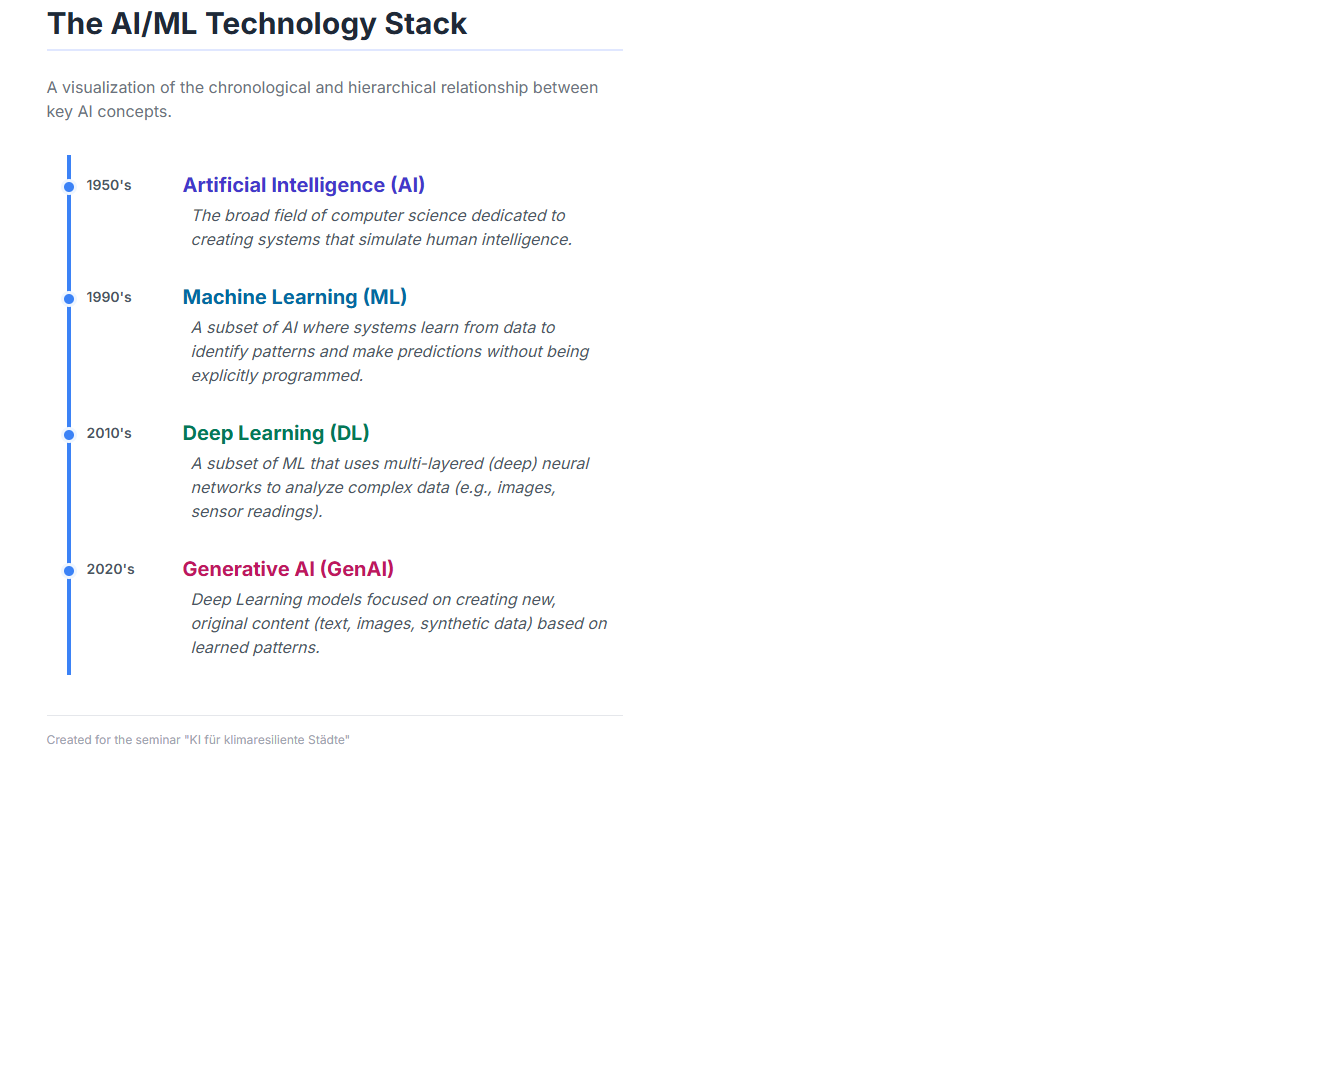
\includegraphics[width=1\textwidth]{images/history_AI_1.png}
    \caption{chronological evolution of AI and ML}
    \label{fig:history_AI}
\end{figure}

\subsection{Focus, Objectives, and Scope}

This seminar paper investigates the transformative potential of Artificial Intelligence (AI), with an 
emphasis on Machine Learning (ML) techniques, to create climate-resilient cities (Smart Cities). The analysis is 
structured around two specific, interconnected applications, forming the scope of this work:
\begin{itemize}
    \item \textbf{AI-Driven Prediction:} The use of ML models, integrating remote sensing (satellite data) and dense sensor networks,
to provide highly accurate, localized, and timely forecasts for key risks such as heatwaves (Hitzewellen) and heavy 
rainfall (Starkregen).

    \item \textbf{Infrastructure Optimization:} The application of AI for the dynamic, real-time control of urban systems, focusing
specifically on rainwater management (e.g., in the context of the "Sponge City" concept) to maximize flood protection
and water conservation.
\end{itemize} 
Through a text-driven analysis of current research, case studies, and expert insights, this work evaluates how these 
robust and adaptive AI systems can significantly enhance urban resilience and outlines the necessary social, economic, 
and technical conditions for their sustainable implementation.
\section{Machine Learning Models}
Building on the theoretical foundation of Artificial Intelligence (AI) described in Section 2.2, this chapter focuses on 
the practical methods and algorithms that enable the implementation of AI in climate-resilient urban systems.
In particular, the emphasis lies on Machine Learning (ML) techniques, which empower predictive and adaptive decision-making 
in Smart Cities. ML provides the computational foundation for analyzing large volumes of climate, environmental, and sensor 
data, and for dynamically optimizing infrastructure responses such as drainage control, energy distribution, and water management.

Although the terms Artificial Intelligence and Machine Learning are often used interchangeably, they refer to distinct concepts. 
Artificial Intelligence is the overarching discipline that aims to simulate human cognitive functions such as reasoning, learning, 
and decision-making. Machine Learning, by contrast, is a subset of AI that enables systems to automatically learn from data and 
improve their performance without being explicitly programmed for each task.
While traditional AI systems rely on rule-based logic — a series of explicit if-then-else statements designed by human 
programmers — ML systems infer these decision rules autonomously by identifying statistical patterns within large datasets.

In the context of Smart Cities and climate resilience, ML algorithms enable data-driven adaptation, allowing infrastructure 
systems to react intelligently to dynamic environmental conditions. Depending on the nature of the learning problem, 
ML approaches are generally grouped into three categories:
\begin{enumerate}
    \item Supervised learning -- models learn from labeled datasets (e.g., historical temperature and rainfall data) to 
    predict future values or classify events such as heatwaves or flooding risks.
    \item Unsupervised learning -- algorithms discover hidden structures in unlabeled data, for example clustering 
    urban areas by micro-climate patterns or detecting anomalies in sensor networks.
    \item Reinforcement Learning (RL) -- agents learn by interacting with the environment and receiving 
    feedback (rewards or penalties); RL can be applied to optimize adaptive control systems such as real-time 
    drainage management or smart grid operations.
\end{enumerate}
\subsection{Mathematical and Engineering Foundations of Machine Learning}
\subsubsection{Pattern Recognition}
In this section we will start by discussing pattern recognition, this has been a key role in enginering and today its used the most in data-science. 
It involves identifying regularities and structures in data and its an important technique when the goal is to classify input data into predefined categories based on similar features.
Multivariable calculus, linear algebra, probability theory, and statistics form the mathematical backbone of machine learning algorithms.\cite{bishop2006pattern}
We will use a very handy example here taken from this book \cite{bishop2006pattern} to illustrate how these mathematical concepts are applied in machine learning.

\begin{figure}[h]
    \centering
    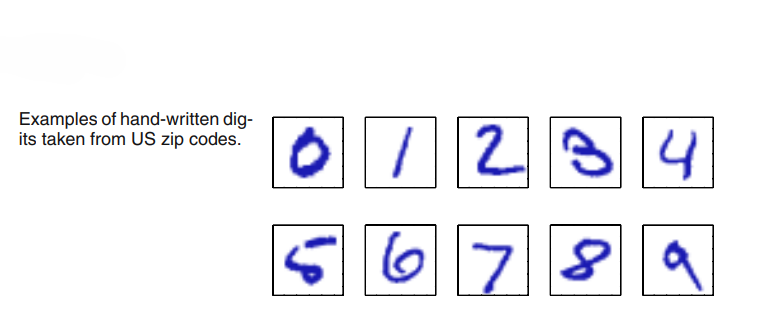
\includegraphics[width=0.8\textwidth]{images/Machine_learning_pixel.png}
    \caption{Analogy between pattern recognition in handwritten digits and climate-resilience modelling. Adapted from \cite{bishop2006pattern}}
    \label{fig:ml_example}
\end{figure}


The challenge of discovering patterns in data has been fundamental to scientific progress for centuries. 
Early examples include how Tycho Brahe’s astronomical observations enabled Kepler to derive the laws of planetary motion, 
laying the foundation for classical mechanics, or how patterns in atomic spectra helped establish quantum theory.

In a modern context, the field of pattern recognition focuses on how computer systems can automatically detect regularities 
within data and use these patterns to perform tasks such as classification or prediction. A common example is the recognition 
of handwritten digits (as shown in Figure 3.x), where each image of a digit can be represented as a 28×28 grid of pixel 
intensities — forming a 784-dimensional input vector.

The goal of the model is to map each input vector $x$ to its correct category, corresponding to one of the digits 0–9 
(see Figure~\ref{fig:ml_example}). Rather than relying on handcrafted rules that describe the shapes of digits — which 
would be extremely complex and error-prone — machine learning methods instead learn these distinctions automatically from data.

In this process, a training set of $N$ labeled examples $\{x_1, \dots, x_N\}$ is used to adjust the parameters of an 
adaptive model so that its predictions $y(x)$ approximate the true target labels $t$. The precision and accuracy of this output function $y(x)$ is determined and improve during 
\emph{training process} also called the \emph{learning phase}. Of course there comes always the need to for the preparation 
of the original dataset, including tasks such as data cleaning, normalization, and augmentation before the actual training process.
The right data representation form is very plays a core role in the success of the model. Once trained, the model can correctly 
classify new, unseen images \emph{(the test set)}, demonstrating its ability to generalize beyond the data it was trained on — a 
key property of successful learning systems (Bishop, 2006).

\subsubsection{Learning Paradigms}

The ability to recognize patterns and structures in data is one of the central goals of machine learning \cite{bishop2006pattern}. 
Before a model can be trained, the raw data usually undergoes a \textbf{pre-processing} or \textbf{feature extraction} step. 
This process aims to simplify the data by removing noise, reducing redundancy, and emphasizing the most relevant information.
For instance, in image-based tasks such as handwritten digit recognition, each image is often resized and centered so that all digits share a similar position and scale. 
Such normalization minimizes variability and makes it easier for algorithms to distinguish between categories. 
In engineering contexts, similar preprocessing may involve standardizing sensor readings, normalizing units, or filtering out measurement noise to prepare the data for learning.

Pre-processing also serves a practical purpose in reducing computational complexity. 
In real-time systems such as video surveillance or autonomous monitoring, the amount of data generated can be extremely large. 
Instead of feeding all raw pixels or raw sensor readings directly into the learning model, \textbf{feature extraction} methods are applied to derive informative yet compact input representations. 
This represents a form of \textbf{dimensionality reduction}, as only a subset of the available information is retained — the part most relevant for the learning task.

Figure~\ref{fig:pattern_example} illustrates the basic concept of a learning problem. 
The blue circles represent individual observations of an input variable \(x\) and its corresponding target variable \(t\). 
The smooth green curve represents the true but unknown function that generated the data. 
The learning algorithm aims to infer this hidden relationship using only the observed data points, allowing it to make predictions for new, unseen inputs. 

\subsubsection*{Polynomial Curve Fitting}

To better understand the process of learning from data, we consider a simple regression problem that illustrates the fundamental ideas behind supervised learning \cite{bishop2006pattern}. 
Assume that we observe a real-valued input variable \(x\) and wish to predict a corresponding real-valued output variable \(t\). 
In practical applications, the true relationship between these quantities is typically unknown, and the observed data often contain random noise. 
For illustration, synthetic data can be generated from a known underlying function, such as \(\sin(2\pi x)\), with added Gaussian noise to simulate natural variability. 
This represents a realistic situation where data exhibit an underlying regularity that we aim to learn, while individual measurements are affected by random disturbances.

Given a training set of \(N\) observed input--output pairs, denoted as 
\[
\mathcal{D} = \{ (x_1, t_1), (x_2, t_2), \dots, (x_N, t_N) \},
\]
our goal is to infer the underlying relationship between \(x\) and \(t\) so that predictions can be made for new inputs. 
One common approach is to fit a \textbf{polynomial function} to the data, expressed as
\[
y(x, \mathbf{w}) = w_0 + w_1x + w_2x^2 + \dots + w_Mx^M = \sum_{j=0}^{M} w_j x^j,
\]
where \(M\) is the \textit{order} of the polynomial, and \(\mathbf{w} = (w_0, w_1, \dots, w_M)^{T}\) represents the set of coefficients. 
Although the function \(y(x, \mathbf{w})\) is nonlinear with respect to the input variable \(x\), it is \textbf{linear in the parameters} \(\mathbf{w}\), and therefore belongs to the family of linear models.

The parameters of the polynomial are determined by minimizing an \textit{error function} that quantifies the discrepancy between the predicted values \(y(x_n, \mathbf{w})\) and the observed target values \(t_n\) in the training data. 
A widely used choice is the \textbf{sum-of-squares error function}, defined as
\[
E(\mathbf{w}) = \frac{1}{2} \sum_{n=1}^{N} \left\{ y(x_n, \mathbf{w}) - t_n \right\}^2.
\]
Minimizing this function with respect to \(\mathbf{w}\) yields the coefficients that best fit the polynomial to the data. 
The factor of \(1/2\) is included for mathematical convenience, as it simplifies later derivative computations. 
This process embodies the core concept of supervised learning: the model parameters are adjusted to reduce the difference between predictions and known targets, allowing the learned function to approximate the true underlying relationship.

In the context of machine learning, this curve-fitting task highlights two critical aspects: 
(1) the need to generalize from a limited number of training examples to unseen inputs, and 
(2) the influence of model complexity \(M\) on the ability of the function to capture meaningful patterns without overfitting the noise in the data. 
These concepts form the foundation for more advanced methods, including neural networks and other nonlinear models, which are explored in later sections.


\begin{figure}[h!]
    \centering
    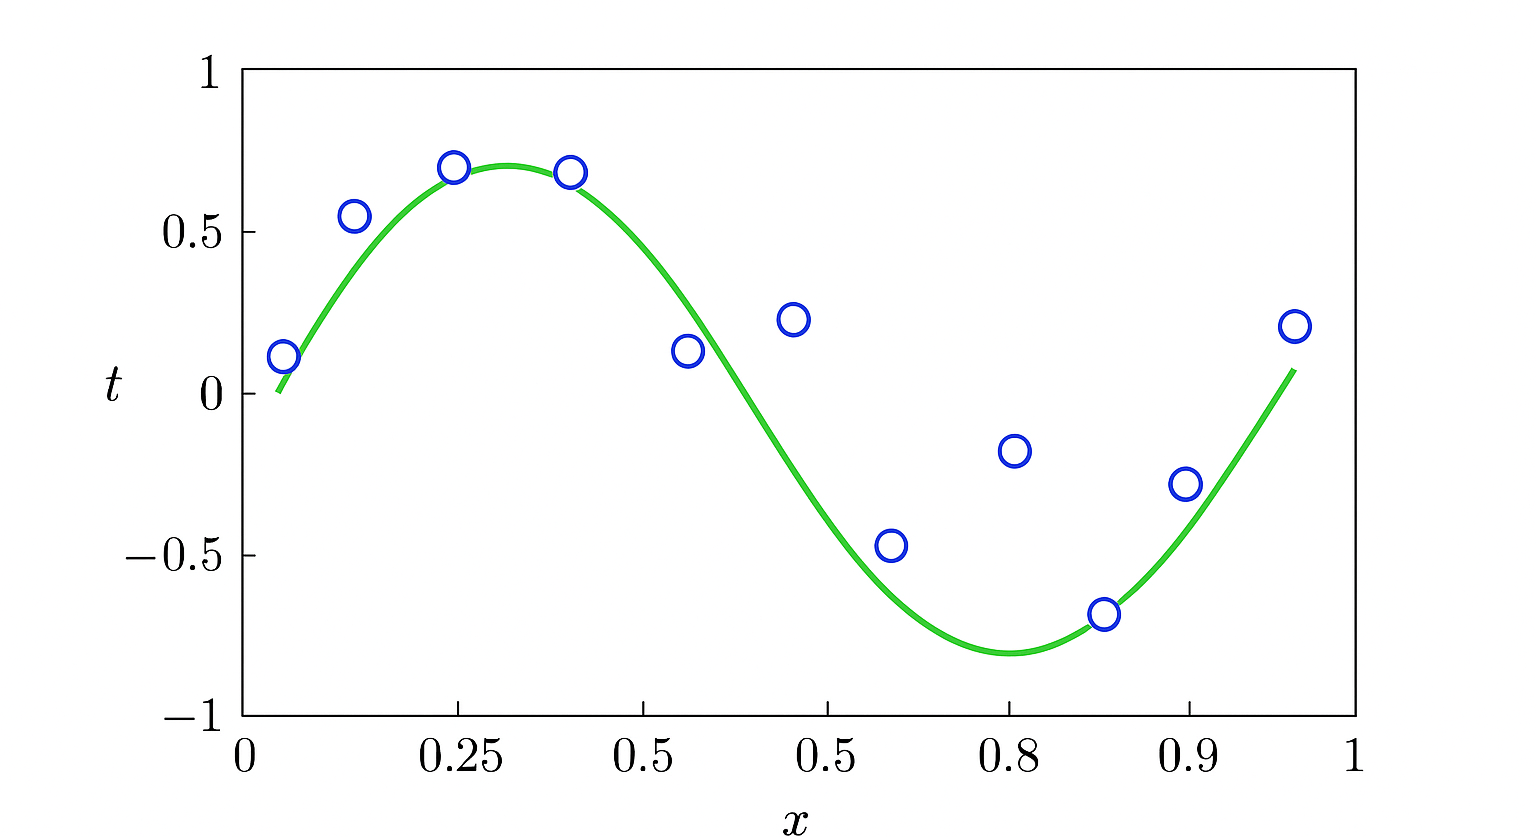
\includegraphics[width=0.75\textwidth]{images/pattern_example_1.png} % changed: correct path and filename (no backslash escapes)
    \caption{Illustration of a supervised learning problem, where the model learns to approximate the underlying function from a limited number of observed data points. Own illustration, inspired by \cite{bishop2006pattern}.}
    \label{fig:pattern_example}
\end{figure}

Depending on the type of data and the objective, machine learning problems can be categorized into three major paradigms \cite{bishop2006pattern}:

\begin{itemize}
    \item \textbf{Supervised Learning:}  
    In this setting, both the input variables and their corresponding target outputs are known.  
    The goal is to learn a mapping function that can predict the output for new inputs.  
    Examples include \textit{classification} tasks (assigning data to discrete categories, such as identifying weather conditions as ``heatwave,'' ``normal,'' or ``storm'') and \textit{regression} tasks (predicting continuous values, such as temperature or rainfall).

    \item \textbf{Unsupervised Learning:}  
    Here, only the input data is available without any labels.  
    The algorithm must find hidden patterns, clusters, or structures within the data.  
    Common techniques include clustering and dimensionality reduction.  
    Such methods are useful for identifying groups of cities with similar climate behavior or for detecting anomalies in environmental sensor networks.

    \item \textbf{Reinforcement Learning (RL):}  
    This approach is based on interaction between an agent and its environment.  
    The agent learns by performing actions and receiving feedback in the form of rewards or penalties.  
    The objective is to find a sequence of actions that maximizes the cumulative reward over time.  
    Reinforcement learning is particularly well suited for dynamic decision-making problems such as adaptive traffic control, smart energy management, or water flow optimization in urban drainage systems \cite{sutton1998reinforcement}.
\end{itemize}

Although these paradigms differ in their data requirements and goals, they share the same mathematical foundation: the optimization of a performance measure or loss function. 
Each algorithm seeks to generalize from observed data to unseen situations, which is crucial for building reliable and adaptive systems in real-world applications.

\subsection{Discrete Probability and Uncertainty}

\begin{figure}[h!]
    \centering
    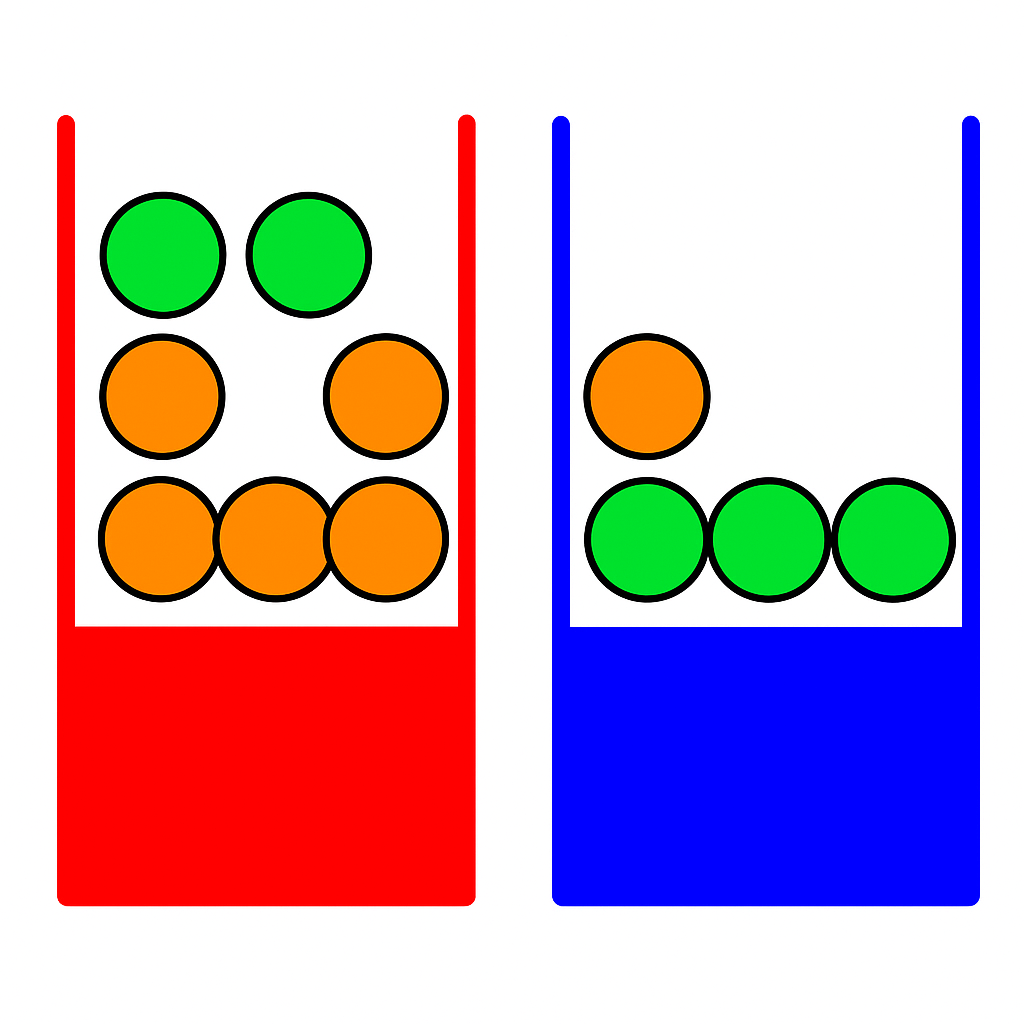
\includegraphics[width=0.6\textwidth]{images/probability_boxes.png}
    \caption{Illustration of the probability example using two boxes. 
    The red box contains 2 apples (green) and 6 oranges (orange), 
    while the blue box contains 3 apples and 1 orange. 
    This example demonstrates the basic concept of random selection and conditional probability. 
    Own illustration, inspired by \cite{bishop2006pattern}.}
    \label{fig:fruit_boxes}
\end{figure}

One of the most important concepts in pattern recognition and machine learning is \textbf{uncertainty}. 
Uncertainty arises naturally in almost all real-world systems due to two main factors: 
(1) measurement noise and (2) limited data availability. 
\textbf{Probability theory} provides a consistent mathematical framework to represent and quantify this uncertainty. 
When combined with decision theory, probability allows us to make optimal predictions even when the available information is incomplete or ambiguous \cite{bishop2006pattern}.

To introduce the fundamental ideas of probability, consider a simple thought experiment involving two boxes, one red and one blue. 
The red box contains two apples and six oranges, while the blue box contains three apples and one orange. 
Suppose we randomly choose one of the boxes and then select one piece of fruit from it. 
After recording which fruit was selected, we return it to the same box and repeat this process many times.

Let the random variable \( B \) represent the chosen box, where \( B = r \) corresponds to the red box and \( B = b \) to the blue box. 
Similarly, let \( F \) denote the fruit type, where \( F = a \) represents an apple and \( F = o \) represents an orange. 
If the red box is chosen 40\% of the time and the blue box 60\% of the time, we can express these probabilities as
\[
p(B = r) = 0.4, \qquad p(B = b) = 0.6.
\]
By definition, all probabilities lie in the interval \([0, 1]\) and must sum to one when representing mutually exclusive outcomes:
\[
p(B = r) + p(B = b) = 1.
\]

With these basic definitions, we can ask more interesting questions, such as:  
“What is the overall probability of selecting an apple?” or  
“Given that we picked an orange, what is the probability that it came from the blue box?”  
Answering such questions requires two essential rules of probability — the \textbf{sum rule} and the \textbf{product rule}.

To derive these, consider two general random variables \( X \) and \( Y \), each capable of taking discrete values \( x_i \) and \( y_j \), respectively. 
If we perform \( N \) trials, and the number of occurrences of both \( X = x_i \) and \( Y = y_j \) is denoted by \( n_{ij} \), then the \textbf{joint probability} is defined as
\[
p(X = x_i, Y = y_j) = \frac{n_{ij}}{N}.
\]
Similarly, the probability of \( X = x_i \) regardless of the value of \( Y \) — known as the \textbf{marginal probability} — is
\[
p(X = x_i) = \frac{c_i}{N},
\]
where \( c_i = \sum_j n_{ij} \).
These relationships form the basis for the sum rule:
\[
p(X = x_i) = \sum_j p(X = x_i, Y = y_j),
\]
and for the product rule, which expresses joint probability in terms of conditional probability:
\[
p(X, Y) = p(Y | X) p(X).
\]
Together, these two rules provide the mathematical foundation for more advanced probabilistic reasoning, including Bayesian inference.

Understanding and applying these principles is important in machine learning, where uncertainty is an inherent part of data modeling. 
For example, when predicting rainfall or temperature in a climate-resilient Smart City system, the measurements obtained from sensors are not exact but follow an underlying probability distribution due to random variations and environmental factors. 
By representing uncertainty probabilistically, we can design models that reason about risk and make more robust, data-driven decisions in uncertain environments.


\subsection{Probability Density for Continuous Variables}

The examples discussed so far have involved discrete random variables, such as selecting a fruit or a box, where probabilities can be expressed as simple fractions of occurrences. 
However, in most real-world engineering applications, the quantities of interest are continuous rather than discrete. 
For instance, temperature, rainfall, or air pressure can take any value within a continuous range. 
In such cases, the concept of probability is expressed not by individual probabilities but by a \textbf{probability density function (PDF)} \cite{bishop2006pattern}.

For a continuous random variable \( x \), the probability of observing a value within a small interval \([x, x + \delta x]\) is given by
\[
p(x) \, \delta x,
\]
where \( p(x) \) is the probability density at point \( x \). 
The density function satisfies the normalization condition
\[
\int_{-\infty}^{\infty} p(x) \, dx = 1,
\]
ensuring that the total probability over all possible outcomes equals one. 
Unlike discrete probabilities, \( p(x) \) itself does not represent the probability of a specific value, since the probability of any exact point in a continuous range is zero. 
Instead, the area under the curve of \( p(x) \) over an interval gives the probability of the variable falling within that range.

A commonly used density function is the \textbf{Gaussian} or \textbf{normal distribution}, defined as
\[
p(x) = \frac{1}{\sqrt{2\pi\sigma^2}} \exp{\left(-\frac{(x - \mu)^2}{2\sigma^2}\right)},
\]
where \( \mu \) is the mean and \( \sigma^2 \) is the variance. 

\begin{figure}[h!]
    \centering
    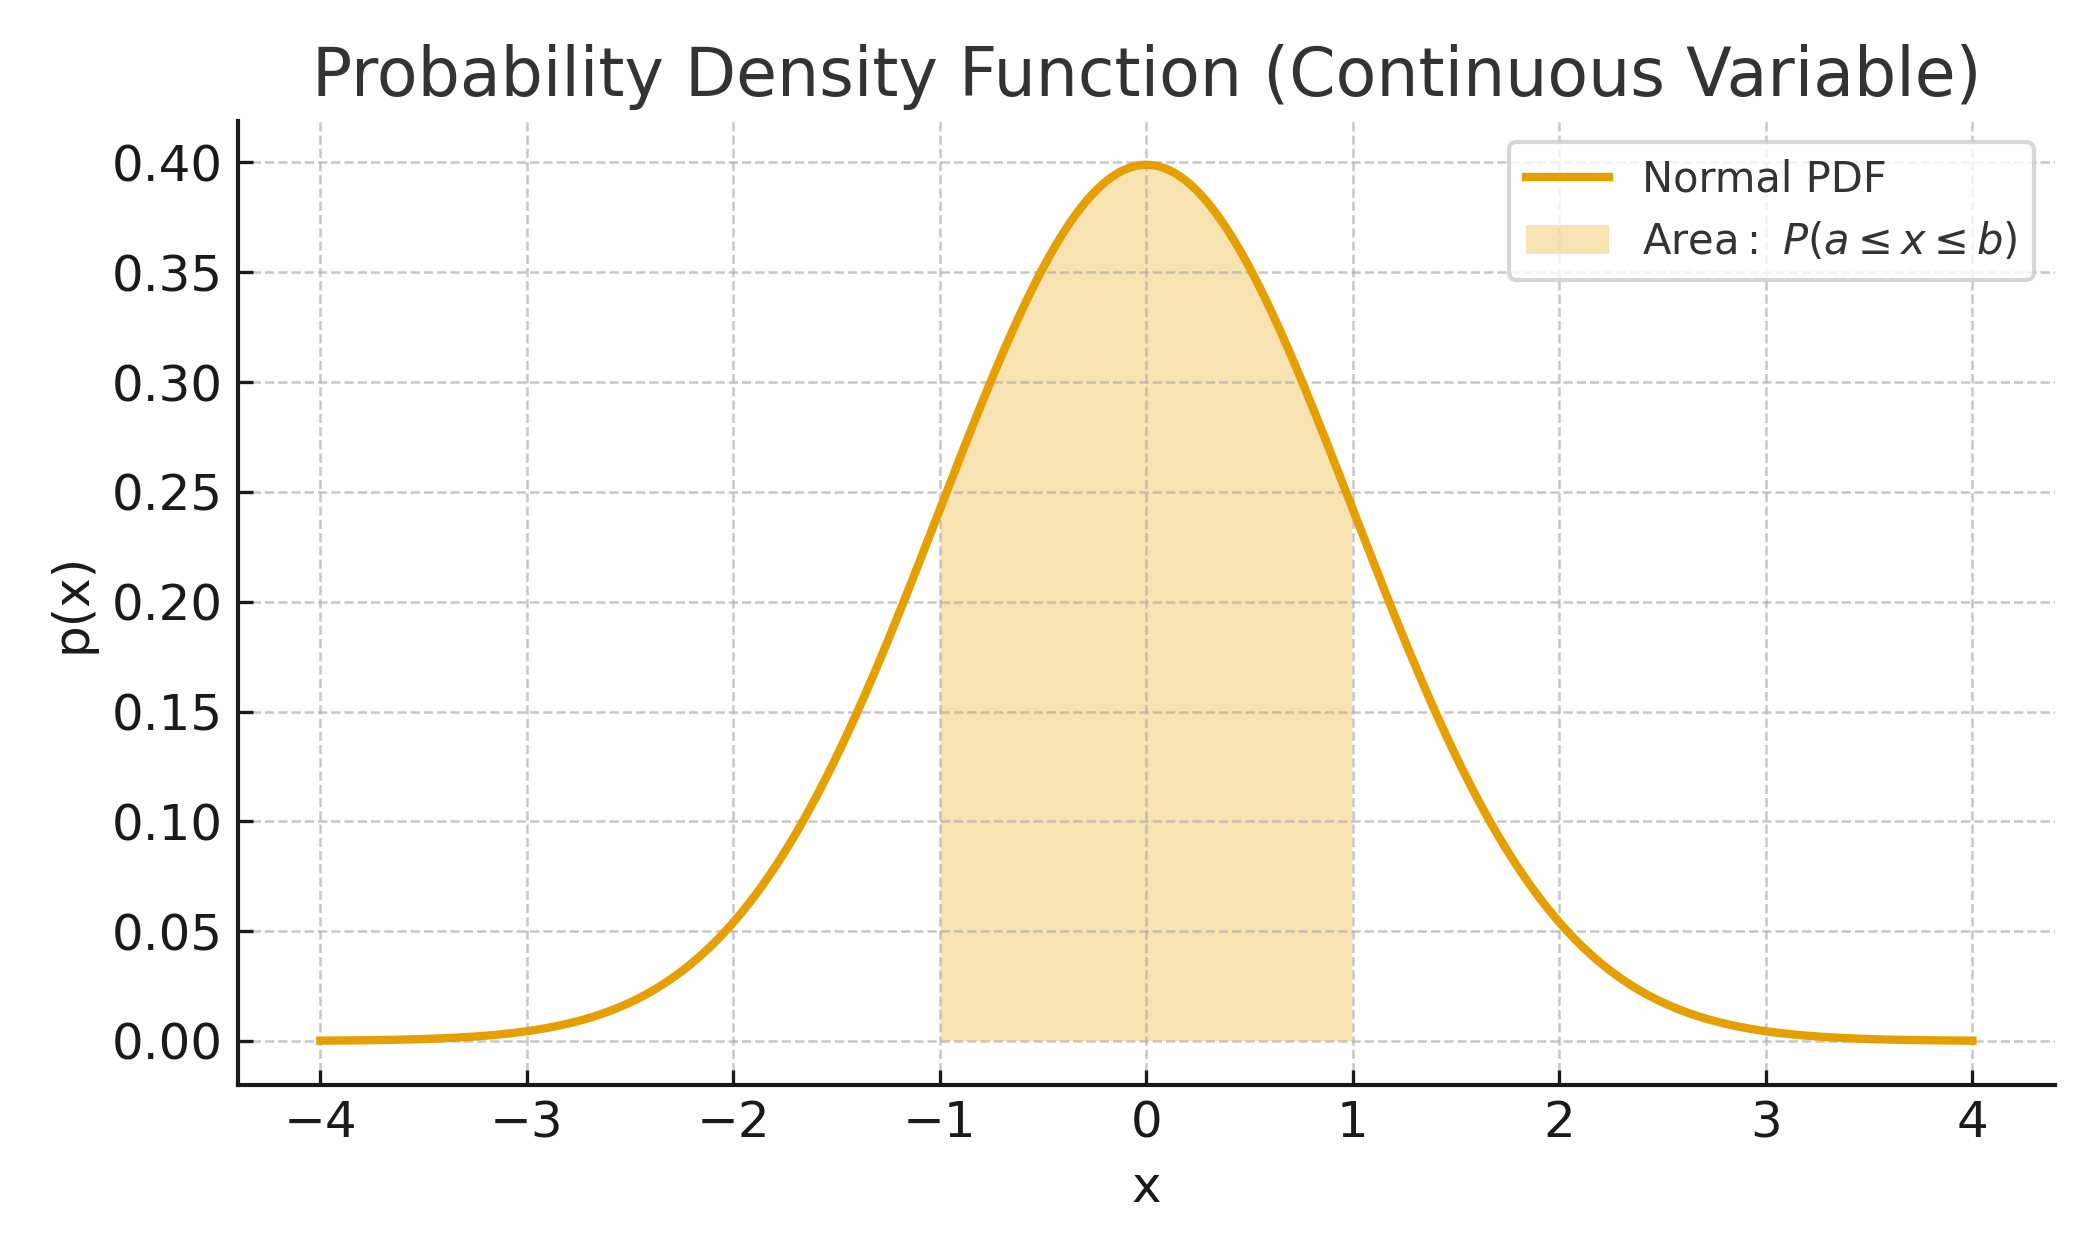
\includegraphics[width=0.7\textwidth]{images/pdf_continuous_density.png}
    \caption{Example of a probability density function for a continuous variable. 
    The shaded area indicates the probability of the variable falling within the interval \(a \le x \le b\).
    Own illustration, inspired by \cite{bishop2006pattern}.}
    \label{fig:pdf_example}
\end{figure}


This distribution is fundamental in machine learning because it models random measurement noise and forms the basis of many probabilistic learning algorithms.

In the context of climate-resilient urban systems, continuous variables such as rainfall intensity or air temperature are naturally modeled using probability densities. 
This enables the prediction of likely outcomes and their associated uncertainties, forming a key component of reliable decision-making in smart infrastructure and environmental monitoring.

\section{Decision Making}

In the previous sections, probability theory was introduced as a framework for representing and reasoning about uncertainty in data. 
However, in many engineering systems, particularly those related to urban infrastructure and climate resilience, we must not only estimate probabilities but also make \textbf{optimal decisions} based on uncertain information. 
\textbf{Decision theory}, when combined with probability, provides the mathematical foundation for choosing actions that minimize risk or cost in uncertain environments \cite{bishop2006pattern}.

\subsection{Decision Theory and Classification}

In general, we observe an input vector \( \mathbf{x} \) — for example, sensor readings from a weather or flood monitoring system — 
and wish to predict an associated outcome \( t \). 
In regression problems, \( t \) may represent a continuous variable such as predicted rainfall or temperature, while in classification 
problems, \( t \) corresponds to discrete classes such as “flood risk,” “heatwave,” or “normal conditions.” 
The joint probability distribution \( p(\mathbf{x}, t) \) expresses all uncertainty associated with these variables. 
Once this distribution is estimated from data, decision theory provides a rule for selecting the most appropriate class or action.

For instance, in an early-warning flood detection system, the input vector \( \mathbf{x} \) might contain real-time measurements 
such as rainfall intensity, river level, and soil moisture. 
Using Bayes’ theorem, we can compute the probability of each event (or class) given these observations:
\[
p(C_k | \mathbf{x}) = \frac{p(\mathbf{x} | C_k)\, p(C_k)}{p(\mathbf{x})}.
\]
Here, \( p(C_k) \) represents the prior likelihood of a flood or normal condition, and \( p(C_k | \mathbf{x}) \) is the updated (posterior) probability based on new sensor data. 
To minimize classification errors, the optimal decision is to select the class with the highest posterior probability — 
a rule known as the \textbf{maximum a posteriori (MAP)} criterion:
\[
\text{Choose class } C_k \text{ if } p(C_k | \mathbf{x}) > p(C_j | \mathbf{x}) \text{ for all } j \neq k.
\]
This principle underlies most AI-based alert systems, allowing them to classify conditions as safe or hazardous based on 
probabilistic evidence.

\subsection{Minimizing Expected Loss}

In practice, not all mistakes have the same impact. 
For example, triggering a false flood alarm may cause minor inconvenience, while failing to issue a warning when a flood 
actually occurs could lead to major infrastructure damage or loss of life. 
To account for this imbalance, decision theory introduces a \textbf{loss function} (or cost function) \( L_{kj} \), which 
specifies the penalty for taking action \( j \) when the true state of the system is \( k \). 
The objective is to minimize the \textbf{expected loss}, or average cost, over all possible outcomes:
\[
E[L] = \sum_{k} \sum_{j} \int_{R_j} L_{kj}\, p(\mathbf{x}, C_k)\, d\mathbf{x}.
\]
Each region \( R_j \) corresponds to a decision rule (for example, “issue alert” or “do nothing”). 
The optimal strategy assigns each input \( \mathbf{x} \) to the decision that minimizes
\[
\sum_{k} L_{kj}\, p(C_k | \mathbf{x}),
\]
thus integrating the likelihood of events with their potential consequences.

This concept generalizes the MAP rule by weighting different types of errors according to their severity. 
In Smart City systems, this approach enables automated infrastructures — such as energy grids, drainage systems, 
or emergency response networks — to balance trade-offs between false alarms and missed detections in a rational, data-driven manner.

\subsection{Decision Theory in Climate-Resilient Smart Cities}

Decision theory provides the final link between predictive machine learning models and actionable responses in climate-resilient 
urban systems. 
Whereas probability and inference quantify uncertainty, decision theory translates those uncertainties into concrete operational actions. 
For instance, an intelligent drainage system may use ML-based rainfall forecasts to decide whether to open flood gates or store 
excess water, while an adaptive power grid may decide how to redistribute load during extreme heat events. 
In each case, the goal is not only to predict environmental changes but also to \textbf{minimize expected loss} — 
in terms of infrastructure risk, resource inefficiency, or public safety — given uncertain information.

By combining probability, learning, and decision theory, modern Smart City frameworks can make data-driven, context-aware, 
and risk-optimized decisions, which are fundamental to enhancing urban climate resilience.


\subsection{Linking Machine Learning to Climate-Resilient Urban Systems}

In the same way that a model can learn to recognize patterns in handwritten digits \cite{bishop2006pattern}, machine learning techniques can also be trained to detect and predict patterns in environmental and climatic data. 
Each city can be viewed as a complex dynamic system generating vast amounts of heterogeneous data --- from weather stations, IoT sensors, and satellite imagery. 
These measurements, such as temperature, rainfall, humidity, and air-pressure readings, can be represented as high-dimensional input vectors, analogous to the pixel intensities in an image. 
The desired outputs, or target variables, might correspond to climate-related outcomes such as flood probability, heatwave intensity, or infrastructure stress levels. 
Through the process of training and optimization, ML models learn the underlying relationships between these inputs and outputs, thereby enabling data-driven prediction and decision-making for urban resilience.

From an engineering perspective, the implementation of such ML models requires the integration of heterogeneous data streams from multiple sources:
\begin{itemize}
    \item \textbf{Meteorological data:} temperature, precipitation, wind, humidity, and solar radiation.
    \item \textbf{Hydrological data:} river levels, soil moisture, and drainage system capacity.
    \item \textbf{Urban infrastructure sensors:} energy consumption, water usage, traffic flow, and air quality.
\end{itemize}

These datasets are pre-processed and fed into supervised learning models such as regression algorithms, random forests, or deep neural networks to predict extreme weather events or infrastructure performance. 
The optimization principle described earlier --- minimizing a loss function \( L(\theta) \) --- is applied to tune model parameters based on historical data. 
Once trained, the model can generalize to unseen conditions, making it suitable for real-time early-warning systems and adaptive resource management in Smart Cities.

For example, deep learning models such as Long Short-Term Memory (LSTM) networks have been successfully applied to predict short-term rainfall intensity from time-series sensor data, enabling drainage systems to adjust flow capacity proactively \cite{kratzert2019towards}. 
Similarly, convolutional neural networks (CNNs) are used for analyzing satellite imagery to identify flood-prone areas or urban heat islands \cite{rolnick2022tackling}. 
These applications demonstrate how ML transforms static urban planning into adaptive, data-driven decision-making systems that enhance climate resilience \cite{mohanty2020ai,li2021sponge}.


\section{Results}
\lipsum[6-7]  % Results section

\section{Discussion}
\lipsum[8-9]  % Discussion of the results

\section{Bibliography}
\printbibliography[heading=none]

% \section{Appendix}
% \lipsum[10]

\end{document}
